% !TEX root = ../main.tex
\chapter{Twitter}
\label{ch:twitter}

\section{Introduction to Twitter}
\label{sec:twitter}

Twitter is a form of so-called microblogging, which is defined as a form of blogging with small-sized pieces of content,
usually text up to a character-count of 200, which, in the case of Twitter, are called Tweets or statuses
(where this thesis will stick to the latter since it is the predominant terminology used in the official documentation~\cite{twitterDocs}).
This enables light-weight, mobile and easy sharing of opinions, status and activities~\cite{Finin2007},
which proved popular among users and lead to rapid adoption and growth~\cite{mcgiboney2009twitter}.

As shown in~\cref{tab:comparison}, the relationships of following users and being followed by users on Twitter is unreciprocated,
which means it requires no active accepting of followers.\\
This leads to only 22.1\% of users who are being followed by someone, also being followed back by that someone~\cite{Kwak2010}.
Although Twitter offers the option to protect ones account, which means followers need to be accepted,
and users can be blocked, thereby denying them seeing ones content, these options are only used in rare cases,
making the form of relationships they represent the exception~\cite{Kwak2010}.\\
The relationship between different kinds of entities present on Twitter can be seen in~\cref{fig:twitter}

% include diagram
\begin{figure}[htb]
    \caption{Simplified diagram of Twitter entity relations}
    \label{fig:twitter}
    \centering
    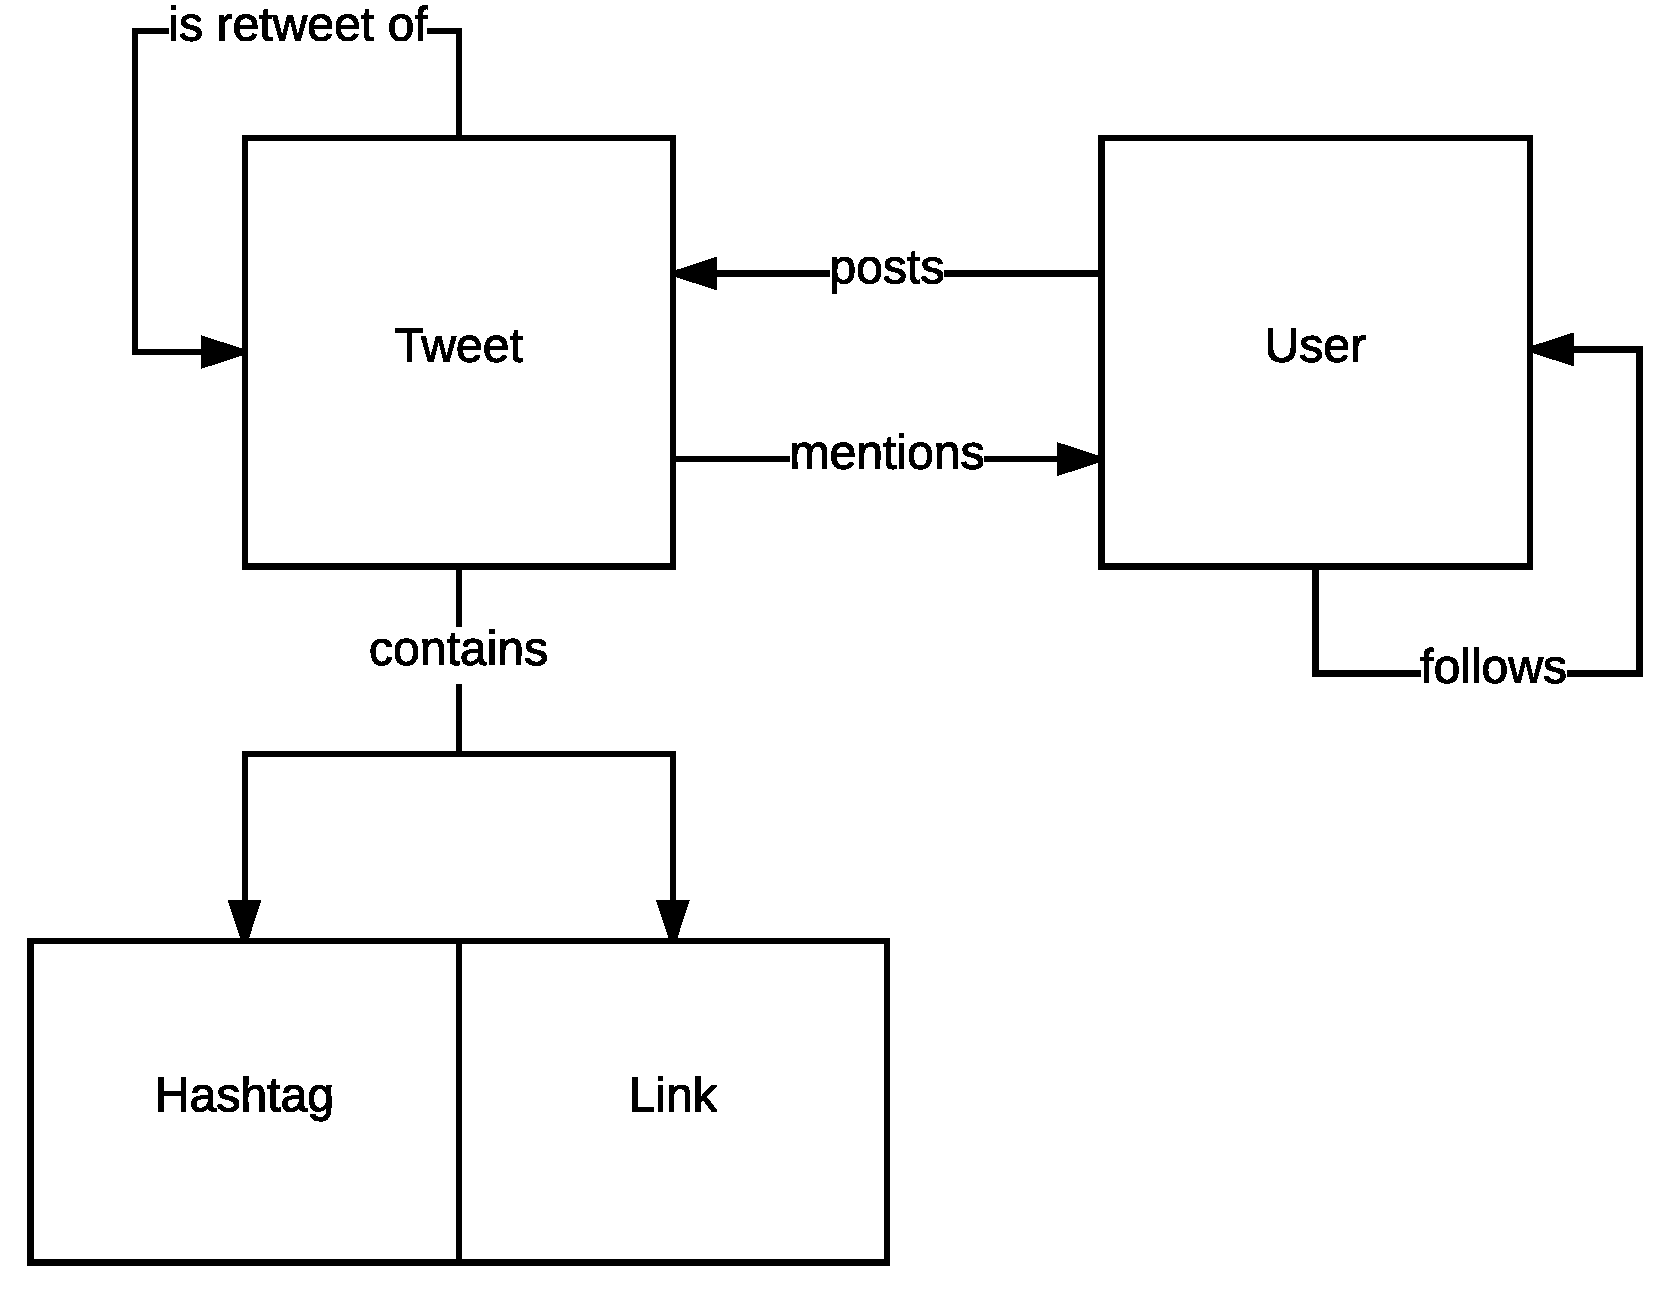
\includegraphics[width=\textwidth]{../figures/twitter_er.pdf}
\end{figure}

This thesis will focus on analyzing statuses in real time.
Statuses on Twitter can not only contain text, but also rich media like images, gifs, or videos, as well as surveys.
The text itself can also contain links, mention other users by containing \texttt{@<user\_name>},
and contain any number of the infamous hashtag (\texttt{\#hashtag}), used to label a status, all while being limited to 140 characters.
A status can also be a so-called retweet of another status, adding to its content and exposing the other status to the retweeting users' followers.
Research shows that statuses are mostly retweeted shortly after they are published, and often lead to chains of retweets,
which not only spreads information fast, but also diffuses it~\cite{Kwak2010}.

For the purpose of this thesis we will only focus on the text of a status and do not assign any special meaning to links,
mentions, hashtags or whether a status is a retweet.\\

\section{The Twitter API}
\label{sec:theApi}

Twitter is offering an API (\textbf{A}pplication \textbf{P}rogramming \textbf{I}nterface),
through which developers and researchers can access machine-readable data,
including the entities shown in~\cref{fig:twitter}, from the platform.
This API transmits data encoded in JSON, and follows the REST-paradigm.
A Python-library called Tweepy, which contains utility functions for interaction with the Twitter API, was used where adequate~\cite{tweepyDocs}.

\subsection{JSON}
\label{subsec:json}

JSON (\textbf{J}ava\textbf{S}cript \textbf{O}bject \textbf{N}otation) is a data format originally conceptualized by ECMA international
for the programming language Javascript.
It was designed to be light-weight, human-readable yet easy for machines to generate and parse.
Due to this, and the fact that it uses conventions familiar to developers of C-like languages,
it has since become a widespread data-interchange format with libraries for parsing and generation in many languages~\cite{jsonDocs}.
A small example for an object in this format can be seen in~\cref{code:json}.


%{
%    "apple": {
%        "calories": 123,
%        "contains_allergens": false
%        "types": ["Braeburh", "Cortland"]
%        "grows_on": "tree"
%    },
%    "hazelnut": {
%        "calories": 12,
%        "contains_allergens": true
%        "grows_on": "bush"
%    },
%}

\begin{figure}
    \caption{A shortened JSON representation of a fictional Twitter status}
    \label{code:json}
    % @formatter:off
    \begin{minted}{json}
    {
        "created_at" : "Fri Jan 20 20:04:05 +0000 2017",
        "id" : "123",
        "text" : "@other_user Hello!",
        "entities" : {
                "hashtags" : [],
                "symbols" : [],
                "user_mentions" : [{
                    "screen_name" : "other_user",
                    "name" : "Other User"}],
                "urls" : [] },
        "user" : {
            "name" : "User",
            "screen_name" : "user"
        }
    }
    \end{minted}
    % @formatter:on
\end{figure}

\subsection{REST}
\label{subsec:rest}

The Twitter API follows the REST (\textbf{RE}presentational \textbf{S}tate \textbf{T}ransfer) paradigm.
The REST-paradigm defines a set of architectural rules to ensure interoperability of distributed systems,
like clients and servers on the internet.
To achieve that, among other things,
it defines a set of methods that specify different kinds of operations that can be performed on data~\cite{Jakl2008}.
The most prevalent methods mentioned in the RFC are listed below~\cite{RFC2616}.

\begin{enumerate}
    \item
    \texttt{GET} - retrieves data identified by the URI (idempotent)
    \item
    \texttt{POST} - request to create a new entity, with the type specified by the URI
    \item
    \texttt{PUT} - request to create an entity identified by the URL, or update it if it exists (idempotent)
    \item
    \texttt{DELETE} - request to delete an entity identified by the URL (idempotent)
\end{enumerate}

There are more methods specified by the RFC~\cite{RFC2616} that will not be used in this thesis.
The resources (also called API endpoints) offered by the Twitter REST-API are rate-limited,
which means any one application or Twitter-user using the API can make a limited number of requests to the API
per 15-minute time window.
Every request send to the API needs to be authenticated,
either as a Twitter user or as an application that can be registered in Twitter's developer console.
There are some resources which can only be accessed when a specific Twitter user authenticates
with the API, because they are user-specific, like publishing a status~\cite{twitterDocs}.
Some examples can be seen in ~\cref{tab:twitter_endpoints}.

\begin{table}
    \caption{A selection of resources offered by the Twitter REST API~\cite{twitterDocs}}
    \label{tab:twitter_endpoints}
    \resizebox{\textwidth}{!}{
    \begin{tabular}{lllll} %
        \toprule
        & & \multicolumn{2}{c}{Authentication} & \\
        \cmidrule{3-4}
        Method
        & URI
        & User
        & Application
        & Description
        \\
        \midrule
        \texttt{GET}
        & \texttt{search/tweets}
        & \cmark
        & \cmark
        & Returns statuses matching a query
        \\
        \midrule
        \texttt{GET}
        & \texttt{direct\_messages}
        & \cmark
        & \xmark
        & Returns direct messages of the authenticated user
        \\
        \midrule
        \texttt{POST}
        & \texttt{statuses/update}
        & \cmark
        & \xmark
        & Posts a status for the authenticated user
        \\
        \bottomrule
    \end{tabular}}
\end{table}

\subsection{Processing Data at Rest and Data in Motion}
\label{subsec:dataAtRest-DataInMotion}

The previous subsection discussed the "data at rest" offered by the Twitter API.
Processing data at rest (not to be confused with REST) means processing data from a persistent data storage, like a database, in batches~\cite{Nandi2015}.
Since this thesis aims to provide analysis in real time, one option would be to request the latest entities in fixed intervals from
Twitters API.

However, this approach would be inefficient, and introduces latency to the analysis,
since events like the posting of statuses can only be analyzed after the next request is answered, not immediately when they occur.
This is amplified by the fact that the number of requests than can be made to the API is limited by the rate-limit,
so a delay would have to be put in between requests.

To analyze events right when they occur, the data has to be processed in motion, meaning ingesting data in real time via a stream~\cite{Nandi2015}.
This thesis aims to process data in motion.
Thankfully, Twitter offers a Streaming API, which is explained in the next subsection.


\subsection{Streaming}
\label{subsec:streaming}

Although the Twitter documentation distinguishes between the REST API for processing data at rest and the the Streaming API for processing data in motion,
the streaming API is also REST-based.
The user sends a HTTP-request to a streaming-endpoint, but the the API doesn't respond and closes the requests,
but instead keeps the connection open and sends successive responses until the connection is closed from the outside.
These responses have the same format as in the REST-API, and represent Twitter entities like statuses or direct messages~\cite{twitterDocs}.
A diagram from the Twitter documentation visualizing this behaviour can be seen in~\cref{fig:twitter_streaming}.

% include diagram
\begin{figure}
    \centering
    \caption{Diagram from the Twitter documentation showing how the Twitter streaming-API works~\cite{twitterDocs}}
    \label{fig:twitter_streaming}
    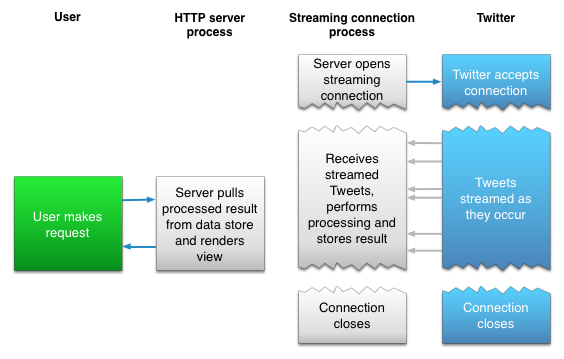
\includegraphics[width=10cm]{../images/twitter_streaming_diagram.png}
\end{figure}

Twitter itself offers 6 different endpoints for 6 different streams, all of which are explained in~\cref{tab:twitter_streams}.

\begin{table}
    \caption{All streams offered by Twitter~\cite{twitterDocs}}
    \label{tab:twitter_streams}
    \resizebox{\textwidth}{!}{%
    \begin{tabular}{llllll} %
        \toprule
        & & & \multicolumn{2}{c}{Authentication} \\
        \cmidrule{4-5}
        Name
        & Method
        & URI
        & User
        & Application
        & Description
        \\
        \midrule
        Filter stream
        & \texttt{POST}
        & \texttt{statuses/filter}
        & \cmark
        & \cmark
        & Streams a random sample of statuses matching the filter setting
        \\
        \midrule
        Sample stream
        & \texttt{GET}
        & \texttt{statuses/sample}
        & \cmark
        & \cmark
        & Streams a random sample of statuses
        \\
        \midrule
        User stream
        & \texttt{GET}
        & \texttt{user}
        & \cmark
        & \xmark
        & Streams all activity regarding the authenticated user
        \\
        \midrule
        Site stream
        & \texttt{GET}
        & \texttt{site}
        & & &
        \\
        \cmidrule{1-3}
        Retweet stream
        & \multicolumn{2}{c}{\textit{Unknown}}
        & \multicolumn{3}{c}{Not publicly available, disregarded}
        \\
        \cmidrule{1-3}
        Firehose
        & \multicolumn{2}{c}{\textit{Unknown}}
        & & &
        \\
        \bottomrule
    \end{tabular}}
\end{table}

This thesis will work with the sample- and filter-stream, since only these are publicly available and do not depend on a specific user,
to give reproducible results.
The main focus will be the sample stream, since it gives a representative sample of all activity on Twitter.
While these streaming endpoints are not rate limited in the number of entities streamed,
they are limited in regards to the number of connection requests any one user or application can make.
To give a feeling for the rate at which statuses will need to be analyzed,
the number of statuses per second for two different streams were recorded over a 10 second period.
The first stream was the sample stream, with the language set to english.
The second stream was the filter stream, tracking only the keyword \texttt{iPhone}, and the language also set to english.
The data was recorded on the 30$^th$ of September 2017.
The results can be seen in~\cref{fig:stream_frequency}.

% include diagram
\begin{figure}
    \centering
    \caption{The number of incoming statuses per second for 2 different streams}
    \label{fig:stream_frequency}
    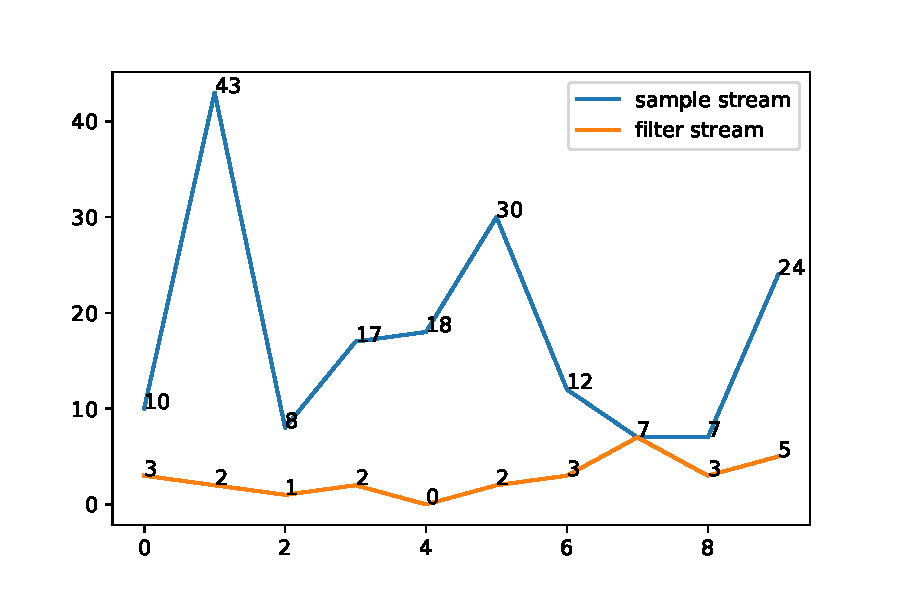
\includegraphics[width=10cm]{../figures/stream_frequencies.pdf}
\end{figure}

It has to be noted that the results are not representative of the share of statuses containing the keyword \texttt{iPhone},
since the Twitter streaming API only sends an indeterminate, small part of all statuses posted~\cite{twitterDocs}.

Compared to the general use-case for Kafka shown in~\cref{fig:kafka}, in this thesis,
every producer will produce events for exactly one topic, with the producer being a specific Twitter stream and the topic beint a unique identifier for it.
The advantage of using the Twitter streaming-API compared to repeatedly polling the REST-API for the use-case of this thesis
is that it is more efficient and has less latency.

\section{The Sanders Dataset}
\label{sec:theSandersDataset}

Since the model used for sentiment analysis will be trained using a supervised approach,
a set of statuses labeled with sentiment was needed.
Evaluation using the comparison in~\cite{Saif2013} showed the Sanders-dataset~\cite{sanders} to be most-suited to train Twitter sentiment analysis models.
At 4347 available statuses, it is large enough to train an accurate model and is hand-labeled instead of relying on, for example, emoticons for labeling, which might be flawed.
Also, Twitter's terms of service forbid the distribution of statuses outside of their API, which ruled out all datasets that did.
Even though the NLTK~\cref{subsec:nltk} contains a Twitter sentiment sample dataset,
there is no information available on how it was collected and labeled, which is why it wasn't considered.
The Sanders-dataset only contains the statuses unique identifier (id), along with the sentiment label ("positive", "negative", "neutral" or "irrelevant").
The existing scripts to hydrate the dataset (meaning to replace the id with the actual status by requesting them from the API) were either slow or deprecated and dysfunctional,
which is why a new script was written.
Unfortunately, due to Twitter's terms of service, no real statuses can be shown, but~\cref{tab:sanders_sample} shows some fictional examples.
The resulting dataset was then filtered to only contain english statuses, which left 2946 statuses.
The distribution of labels on the dataset can be seen in~\cref{fig:sanders_sentiment}.

The statuses were collected using the search terms "@apple", "\#google", "\#microsoft" and "\#twitter",
which not only renders them unusable to create a topic model since that makes them highly topical,
but might also negatively impact the ability of sentiment analysis models trained on them to generalize over other data.
Furthermore, of the remaining english statuses, only 431 and 481 were labeled as positive and negative respectively,
which might be too few to train an accurate model.
This will be explored further in~\cref{ch:sentimentAnalysis}.

\begin{table}[t]
    \begin{minipage}[t]{.56\textwidth }
        \captionof{table}{Some fictional statuses with labels}
        \label{tab:sanders_sample}
        \centering
        \resizebox{\textwidth}{!}{%
        \begin{tabular}{lllll} %
            \toprule
            Text
            & Sentiment Label
            \\
            \midrule
            Lmao I had a funny argument with Siri @Apple
            & \texttt{positive}
            \\
            My \#iPad crashes constantly since the update.
            & \texttt{negative}
            \\
            Can anyone recommend me an app for my iPhone?
            & \texttt{neutral}
            \\
            Apple stellt neues iPhone vor \textit{(non-english)}
            & \texttt{irrelevant}
            \\
            \bottomrule
        \end{tabular}}
    \end{minipage}%
    \hfill
    \begin{minipage}[t]{.4\textwidth}
        \centering
        \captionof{figure}{Sanders dataset label distribution}
        \label{fig:sanders_sentiment}
        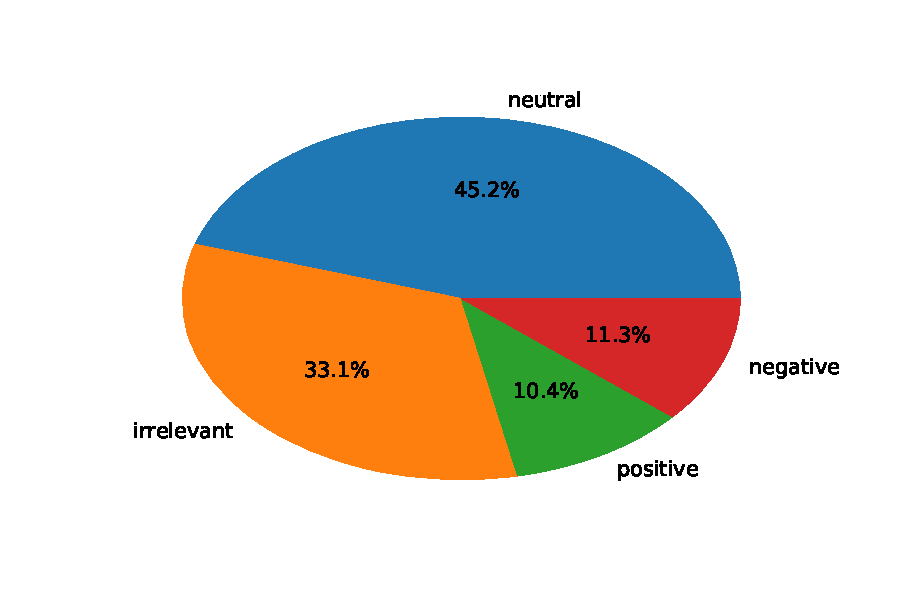
\includegraphics[width=\textwidth]{../figures/sanders_sentiment.pdf}
    \end{minipage}
\end{table}

\section{The Streaming Sample Dataset}
\label{sec:streamingSampleDataset}

Another dataset was collected by streaming the sample stream described in~\cref{subsec:streaming},
again only keeping english tweets.
The statuses were collected on the 18$^{th}$ of august 2017.
The statuses received via the stream were written to a database until 7000 statuses were collected.
This dataset will be used for (unsupervised) topic modeling, since it is representative of all activity on Twitter.
A wordcloud of the statuses collected from the sample stream can be seen in~\cref{fig:wordloud_pre}.

Some of the biggest "words" in the wordcloud are "RT", "it" and "be",
or even some digits, which have no informativeness with regards to sentiment or topic,
demonstrating the necessity of preprocessing, shown in the next chapter.

\section{Preprocessing and Tokenization}
\label{sec:preprocessingAndTokenization}

There are now 2 datasets of statuses that are filtered by language but still raw.
Since the quality of the results will depend on the quality of the data,
these datasets now need to be preprocessed.
In this case that means removing all elements of text that have no influence on topic and sentiment and make
modeling and analysis unnecessarily difficult.\\
Furthermore, since all the algorithms that will be used later on are bag-of-words algorithms,
which means they disregard the order of words in text, a tokenization function needs to be created
to split sentences in the right places and only keep tokens (terms, words) relevant for modeling and analysis.\\
At this point it is important to mention that while the tokenization does not, strictly speaking, tokenize the documents,
but rather splits them into terms, this thesis will stick to the NLTK's~\cite{nltkDocs} nomenclature, and call the terms tokens.\\
To achieve consistent results, the same preprocessing and tokenization functions need to be used for all models, analyses and datasets.
The following steps were taken.

\begin{enumerate}
    \item Preprocessing
    \begin{enumerate}
        \item All URL's were removed by using a regular expression matching everything from "http" up to the next whitespace
        \item All punctuation as well as the Twitter-specific characters \texttt{@} and \texttt{\#} were removed
        \item The text was split at whitespace using the \texttt{\\s} regular expression
        \item All elements that contained anything but latin letters were discarded
    \end{enumerate}
    \item Tokenization
    \begin{enumerate}
        \item The text is split into tokens using the whitespace regular expression again
        \item Terms of length 1 are removed
        \item Terms that can be found in NLTK's stopwords list for the english language
        (containing a fixed selection of terms with low informativeness for bag-of-words algorithms),
        were removed. \textit{(This only applies to topic modeling)}
        \item Terms that can be found in an additional self-devised stopwords list specific to this case were removed
    \end{enumerate}
\end{enumerate}

The Python implementation of these functions can be found in the Appendix in~\cref{sec:preprocessingAndTokenizationFunctionFactories}.

While some approaches to removing terms with low informativeness rely on removing terms that occur in too many or too few documents,
in this thesis, a stopword list is used,
since only english statuses will be considered, and extensive stopword lists exit for the english language~\cite{Porter2001}.
The change to the wordcloud of the statuses collected from the sample stream after preprocessing and tokenization (including stopword removal) can be seen in~\cref{fig:wordloud_post}.

\begin{figure}
    \centering
    \caption{Wordcloud of the statuses collected from the sample stream}
    \label{fig:test}
    \begin{subfigure}{.5\textwidth}
        \centering
        \caption{Before preprocessing and tokenization}
        \label{fig:wordloud_pre}
        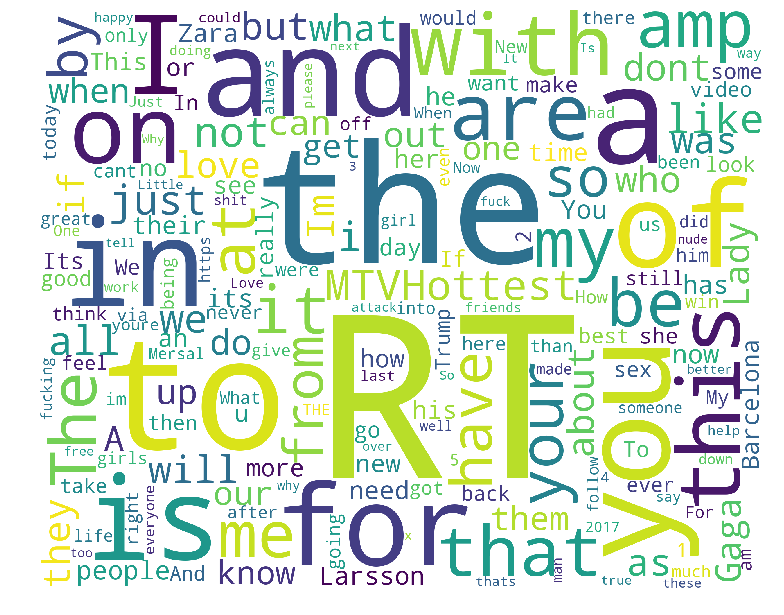
\includegraphics[width=\textwidth]{../images/wordcloud_pre.png}
    \end{subfigure}%
    \begin{subfigure}{.5\textwidth}
        \centering
        \caption{After preprocessing and tokenization}
        \label{fig:wordloud_post}
        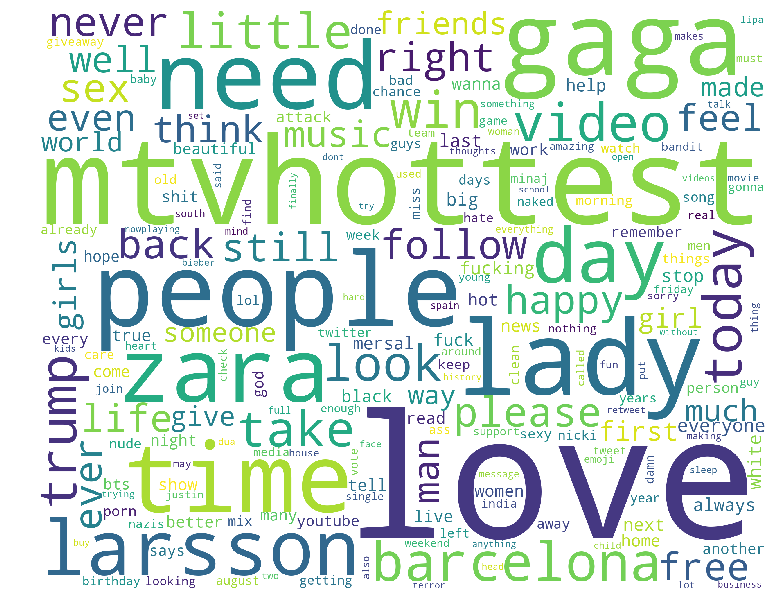
\includegraphics[width=\textwidth]{../images/wordcloud_post.png}
    \end{subfigure}
\end{figure}